\documentclass[fleqn]{beamer}\usepackage[]{graphicx}\usepackage[]{color}
% maxwidth is the original width if it is less than linewidth
% otherwise use linewidth (to make sure the graphics do not exceed the margin)
\makeatletter
\def\maxwidth{ %
  \ifdim\Gin@nat@width>\linewidth
    \linewidth
  \else
    \Gin@nat@width
  \fi
}
\makeatother

\definecolor{fgcolor}{rgb}{0.345, 0.345, 0.345}
\newcommand{\hlnum}[1]{\textcolor[rgb]{0.686,0.059,0.569}{#1}}%
\newcommand{\hlstr}[1]{\textcolor[rgb]{0.192,0.494,0.8}{#1}}%
\newcommand{\hlcom}[1]{\textcolor[rgb]{0.678,0.584,0.686}{\textit{#1}}}%
\newcommand{\hlopt}[1]{\textcolor[rgb]{0,0,0}{#1}}%
\newcommand{\hlstd}[1]{\textcolor[rgb]{0.345,0.345,0.345}{#1}}%
\newcommand{\hlkwa}[1]{\textcolor[rgb]{0.161,0.373,0.58}{\textbf{#1}}}%
\newcommand{\hlkwb}[1]{\textcolor[rgb]{0.69,0.353,0.396}{#1}}%
\newcommand{\hlkwc}[1]{\textcolor[rgb]{0.333,0.667,0.333}{#1}}%
\newcommand{\hlkwd}[1]{\textcolor[rgb]{0.737,0.353,0.396}{\textbf{#1}}}%
\let\hlipl\hlkwb

\usepackage{framed}
\makeatletter
\newenvironment{kframe}{%
 \def\at@end@of@kframe{}%
 \ifinner\ifhmode%
  \def\at@end@of@kframe{\end{minipage}}%
  \begin{minipage}{\columnwidth}%
 \fi\fi%
 \def\FrameCommand##1{\hskip\@totalleftmargin \hskip-\fboxsep
 \colorbox{shadecolor}{##1}\hskip-\fboxsep
     % There is no \\@totalrightmargin, so:
     \hskip-\linewidth \hskip-\@totalleftmargin \hskip\columnwidth}%
 \MakeFramed {\advance\hsize-\width
   \@totalleftmargin\z@ \linewidth\hsize
   \@setminipage}}%
 {\par\unskip\endMakeFramed%
 \at@end@of@kframe}
\makeatother

\definecolor{shadecolor}{rgb}{.97, .97, .97}
\definecolor{messagecolor}{rgb}{0, 0, 0}
\definecolor{warningcolor}{rgb}{1, 0, 1}
\definecolor{errorcolor}{rgb}{1, 0, 0}
\newenvironment{knitrout}{}{} % an empty environment to be redefined in TeX

\usepackage{alltt}

% \usefonttheme[onlylarge]{structuresmallcapsserif}
\usefonttheme[onlysmall]{structurebold}
\usepackage[normalem]{ulem} % use normalem to protect \emph
\newcommand\hl{\bgroup\markoverwith
  {\textcolor{yellow}{\rule[-.5ex]{2pt}{2.5ex}}}\ULon}
\usepackage{amsmath,amssymb}
\usepackage{booktabs}
\usepackage{graphicx}
\usepackage{longtable}
\usepackage{lscape}
\usepackage[authoryear]{natbib}
\usepackage{array}
\usepackage{listings}
\usepackage{wasysym}
\usepackage{url}
\usepackage{multirow}
\usepackage{color}
\usepackage{qtree}
\usepackage{inconsolata}
\usepackage{framed}
\definecolor{shadecolor}{rgb}{1,0.8,0.3}
\usepackage[justification=centering]{caption}
\captionsetup{compatibility=false}
\usepackage{subcaption}
\usepackage{xcolor}
\usepackage{hyperref}
\hypersetup{colorlinks=true,linkcolor=blue}
\usepackage[space]{grffile}
\usefonttheme[onlymath]{serif}
% \usepackage{tikz}
% \usetikzlibrary{calc,matrix}
\usepackage{sgame}
\usepackage{tikz}
\usetikzlibrary{trees}

\mode<presentation>
%\usetheme{Frankfurt}
\usetheme{boxes}
\usecolortheme{beaver}
%\usetheme{Singapore}
%\usetheme{Hannover}

\beamertemplatenavigationsymbolsempty
\setbeamertemplate{blocks}[rounded]
\newenvironment<>{block_code}[1]{%
  \setbeamercolor{block title}{fg=white,bg=black}%
  \begin{block}#2{#1}}{\end{block}}

%===================================
% Coloring change
%===================================
\definecolor{darkred}{rgb}{0.8,0,0}
\setbeamercolor{block title}{fg=darkred,bg=structure.fg!20!bg!50!bg}
\setbeamercolor{block body}{use=block title,bg=block title.bg}

\title{Simple Univariate Regression: Part 2}
\author{Taro Mieno}
\everymath{\displaystyle}
\IfFileExists{upquote.sty}{\usepackage{upquote}}{}
\begin{document}
\begin{frame}
\titlepage
\end{frame}





%===================================
% R implementation
%===================================

\begin{frame}[c]
  \frametitle{Deriving the Ordinary Least Squares (OLS) estimates}
  \begin{enumerate}
    \item You have collected data with $n$ observations on $y$  and $x$
    \item This random sample is denoted as $\{(y_i,x_i):i=1,\dots,n\}$
    \item For each $i$, we can write:
    \begin{align}
        y_i=\beta_0+\beta_1 x_i + u_i \notag
    \end{align}
  \end{enumerate}
\end{frame}

\begin{frame}[c]
  \frametitle{The data set and model}
  \begin{block}{Objective}
    Estimate the impact of lot size on house price
  \end{block}

  \begin{block}{Model}
  \begin{align*}
  price_i = \beta_0 + \beta_1 lotsize_i+u_i
  \end{align*}
  \begin{itemize}
    \item $price_i$: house price (\$) of house $i$
    \item $lotsize_i$: lot size of house $i$
    \item $u_i$: error term (everything else) of house $i$
  \end{itemize}
  \end{block}
\end{frame}

\begin{frame}[c,fragile]
  \frametitle{Data set we are going to use}
  \begin{block_code}{R code: Loading a data set}
  \footnotesize{
\begin{knitrout}
\definecolor{shadecolor}{rgb}{0.969, 0.969, 0.969}\color{fgcolor}\begin{kframe}
\begin{alltt}
  \hlcom{#--- load the AER package  ---#}
  \hlkwd{library}\hlstd{(AER)} \hlcom{# load the AER package}

  \hlcom{#--- load the HousePrices data set ---#}
  \hlkwd{data}\hlstd{(HousePrices)} \hlcom{# load}

  \hlcom{#--- take a look ---#}
  \hlkwd{head}\hlstd{(HousePrices[,}\hlnum{1}\hlopt{:}\hlnum{5}\hlstd{])}
\end{alltt}
\begin{verbatim}
  price lotsize bedrooms bathrooms stories
1 42000    5850        3         1       2
2 38500    4000        2         1       1
3 49500    3060        3         1       1
4 60500    6650        3         1       2
5 61000    6360        2         1       1
6 66000    4160        3         1       1
\end{verbatim}
\end{kframe}
\end{knitrout}
  }
  \end{block_code}
\end{frame}

\begin{frame}[c]
  \frametitle{Random sample and regression}

\begin{columns}[onlytextwidth]
  \begin{column}{0.7\textwidth}
\only<1-1>{
\begin{knitrout}
\definecolor{shadecolor}{rgb}{0.969, 0.969, 0.969}\color{fgcolor}

{\centering \includegraphics[width=3in,height=3in]{figure/fig_2_sample-1} 

}



\end{knitrout}
}

\only<2-2>{
\begin{knitrout}
\definecolor{shadecolor}{rgb}{0.969, 0.969, 0.969}\color{fgcolor}

{\centering \includegraphics[width=3in,height=3in]{figure/fig_2_reg-1} 

}



\end{knitrout}
}
  \end{column}
  \begin{column}{0.3\textwidth}
    \only<2-2>{
    \begin{itemize}
      \item We want to draw a line like this, the slope of which is an estimate of $\beta_1$
      \item A way: Ordinary Least Squares (OLS)
    \end{itemize}

    }
  \end{column}
​\end{columns}
\end{frame}


\begin{frame}[c]
  \frametitle{Before talking about OLS}
  \begin{block}{Residuals}
  For particular values of $\hat{\beta}_0$ and $\hat{\beta}_1$ you pick, the modeled value of $y$ for individual $i$ is $\hat{\beta}_0 + \hat{\beta}_1 x_i$.\\\vspace{0.6cm}

  Then, the residual for individual $i$ is:
  \begin{align*}
     \hat{u}_i =  y_i - (\hat{\beta}_0 + \hat{\beta}_1 x_i)
  \end{align*}
  That is, residual is the observed value of the dependent variable less the value of modeled part. For different values of $\hat{\beta}_0$ and $\hat{\beta}_1$, you have a different value of residual.
  \end{block}

\end{frame}

\begin{frame}[c,fragile]
  \frametitle{Residuals}

\begin{columns}[onlytextwidth]
  \begin{column}{0.7\textwidth}
\only<1-1>{
\begin{knitrout}
\definecolor{shadecolor}{rgb}{0.969, 0.969, 0.969}\color{fgcolor}

{\centering \includegraphics[width=3in,height=3in]{figure/fig_reg_line-1} 

}



\end{knitrout}
}

\only<2-2>{
\begin{knitrout}
\definecolor{shadecolor}{rgb}{0.969, 0.969, 0.969}\color{fgcolor}

{\centering \includegraphics[width=3in,height=3in]{figure/fig_reg_line_2-1} 

}



\end{knitrout}
}
  \end{column}
  \begin{column}{0.3\textwidth}
    \only<1-1>{
    \begin{itemize}
      \item $\hat{\beta}_0=70000$
      \item $\hat{\beta}_1=3.8$
    \end{itemize}
    }
    \only<2-2>{
    \begin{itemize}
      \item $\hat{\beta}_0=20000$
      \item $\hat{\beta}_1=7$
    \end{itemize}
    }
  \end{column}
​\end{columns}
\end{frame}

\begin{frame}[c]
  \frametitle{OLS}

  \begin{block}{Idea}
    Let's find the value of $\beta_0$ and $\beta_1$ that minimizes the squared residuals!
  \end{block}
   \begin{block}{Mathematically}
   \vspace{-0.6cm}
   \begin{align}
       Min_{\hat{\beta}_0,\hat{\beta}_1} \sum_{i=1}^n \hat{u}_i^2, \notag
   \end{align}
   where $\hat{u}_i=y_i-(\hat{\beta}_0+\hat{\beta}_1 x_i)$
   \end{block}
\end{frame}

\begin{frame}[c]
  \frametitle{Ordinary Least Squares (OLS): Visualization}

\begin{knitrout}
\definecolor{shadecolor}{rgb}{0.969, 0.969, 0.969}\color{fgcolor}

{\centering 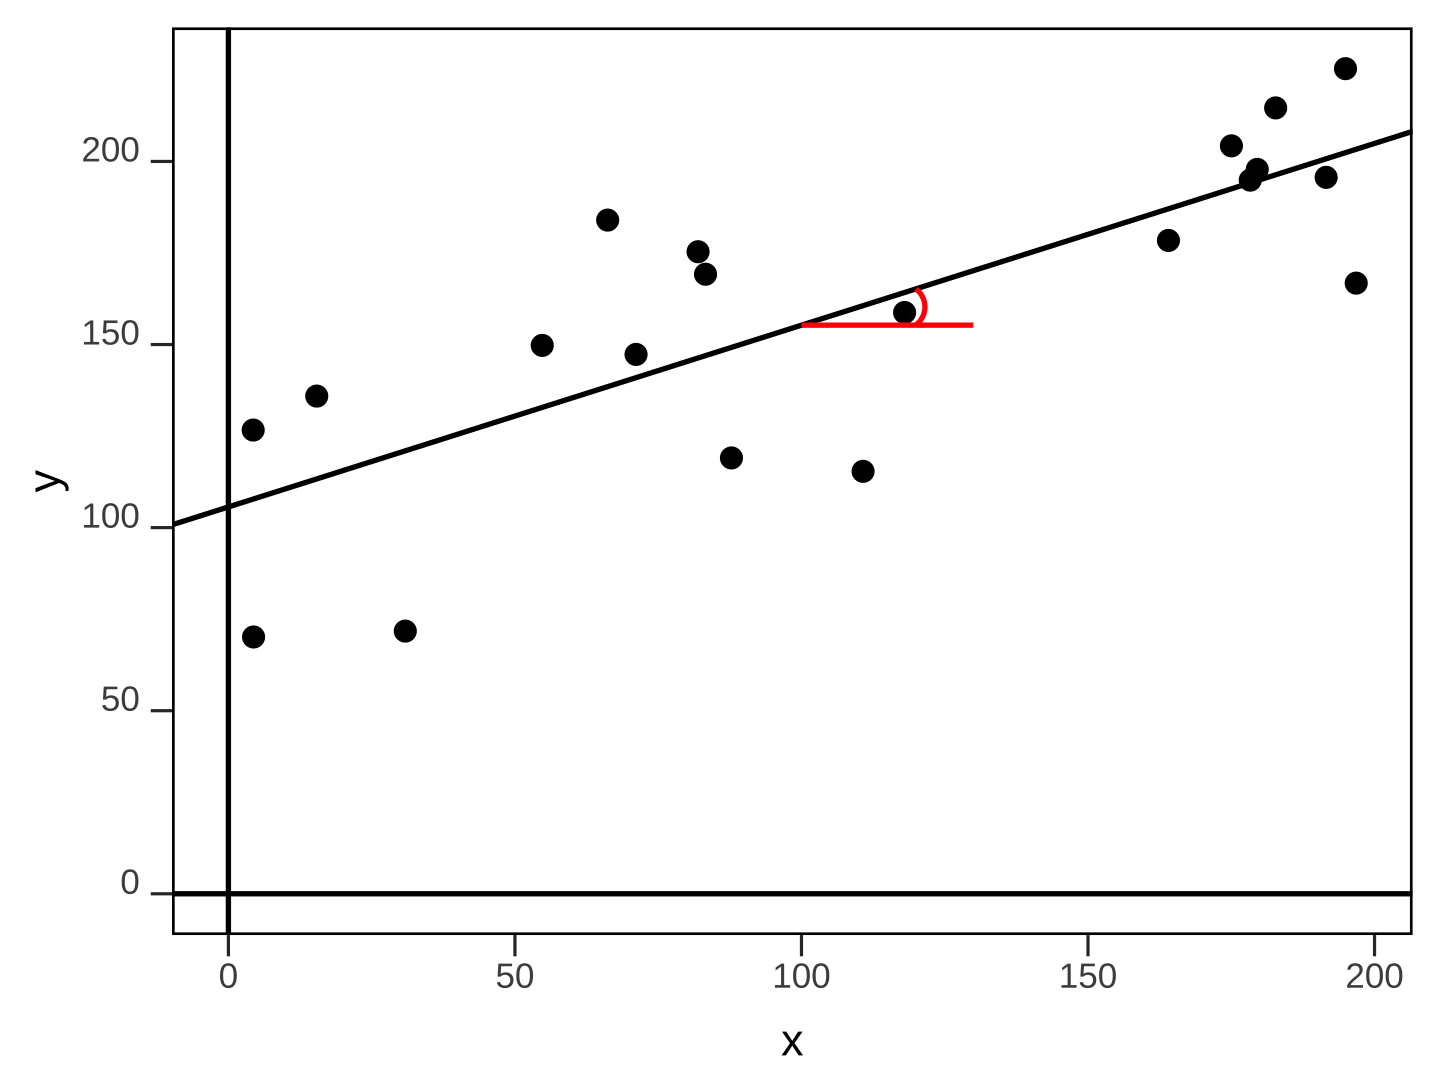
\includegraphics[width=3in,height=3in]{figure/ols-1} 

}



\end{knitrout}
\end{frame}

\begin{frame}[c]
  \frametitle{OLS}
  \begin{itemize}
     \item Why do we square the residuals, and then sum them up together? What's gonna happen if you just sum up residuals?
     \item How about taking the absolute value of residuals, and then sum them up?
   \end{itemize}
\end{frame}

\begin{frame}[c]
  \frametitle{Deriving OLS estimates }
   \begin{align}
       Min_{\hat{\beta}_0,\hat{\beta}_1} \sum_{i=1}^n [y_i-(\hat{\beta}_0+\hat{\beta}_1 x_i)]^2, \notag
   \end{align}

   \begin{block}{Steps}
     \begin{enumerate}
       \item partial differentiation of the objective function with respect to $\hat{\beta}_0$ and $\hat{\beta}_1$
       \item solve for $\hat{\beta}_0$ and $\hat{\beta}_1$
     \end{enumerate}
   \end{block}
\end{frame}

\begin{frame}[c]
  \frametitle{OLS derivation: FOC}
  \begin{align}
       Min_{\hat{\beta}_0,\hat{\beta}_1} \sum_{i=1}^n [y_i-(\hat{\beta}_0+\hat{\beta}_1 x_i)]^2, \notag
   \end{align}
   \begin{block}{FOC}
   \vspace{-0.6cm}
     \begin{align*}
       \frac{\partial }{\partial \hat{\beta}_0}=& 2\sum_{i=1}^n [y_i-(\hat{\beta}_0+\hat{\beta}_1 x_i)]=0 \\
       \frac{\partial }{\partial \hat{\beta}_1}=& 2\sum_{i=1}^n x_i\cdot [y_i-(\hat{\beta}_0+\hat{\beta}_1 x_i)]=0
    \end{align*}
   \end{block}
\end{frame}

\begin{frame}[c]
  \frametitle{OLS derivation: Blank Sheet 1}

\end{frame}

\begin{frame}[c]
  \frametitle{OLS derivation: Blank Sheet 2}

\end{frame}


\begin{frame}[c]
  \frametitle{OLS}
  \begin{block}{OLS estimators: analytical formula}
    \begin{align*}
      \hat{\beta}_1 = & \frac{\sum_{i=1}^n(x_i-\bar{x})(y_i-\bar{y})}{\sum_{i=1}^n(x_i-\bar{x})^2}\\
      \hat{\beta}_0 = & \bar{y}-\hat{\beta}_1 \bar{x}
    \end{align*}
  \end{block}

  \only<2->{\begin{block}{Estimators}
    Specific \textcolor{blue}{rules} to use available data once you get the data
  \end{block}}

  \only<3->{\begin{block}{Estimates}
    Numbers you get once you plug values (your data) into the formula
  \end{block}}

\end{frame}

\begin{frame}[c,fragile]
  \frametitle{OLS demonstration in R}
  \begin{block}{Model}
  \vspace{-0.6cm}
    \begin{align*}
      \hat{\beta}_1 = & \frac{\sum_{i=1}^n(x_i-\bar{x})(y_i-\bar{y})}{\sum_{i=1}^n(x_i-\bar{x})^2}\\
      \hat{\beta}_0 = & \bar{y}-\hat{\beta}_1 \bar{x}
    \end{align*}
  \end{block}
  \begin{block_code}{R code: hard way}
  \scriptsize{
\begin{knitrout}
\definecolor{shadecolor}{rgb}{0.969, 0.969, 0.969}\color{fgcolor}\begin{kframe}
\begin{alltt}
  \hlstd{y} \hlkwb{<-} \hlstd{HousePrices}\hlopt{$}\hlstd{price}
  \hlstd{x} \hlkwb{<-} \hlstd{HousePrices}\hlopt{$}\hlstd{lotsize}

  \hlcom{#--- beta_1 ---#}
  \hlstd{b1_num} \hlkwb{<-} \hlkwd{sum}\hlstd{((x}\hlopt{-}\hlkwd{mean}\hlstd{(x))}\hlopt{*}\hlstd{(y}\hlopt{-}\hlkwd{mean}\hlstd{(y)))}
  \hlstd{b1_denom} \hlkwb{<-} \hlkwd{sum}\hlstd{((x}\hlopt{-}\hlkwd{mean}\hlstd{(x))}\hlopt{^}\hlnum{2}\hlstd{)}
  \hlstd{b1} \hlkwb{<-} \hlstd{b1_num}\hlopt{/}\hlstd{b1_denom}
  \hlstd{b1}
\end{alltt}
\begin{verbatim}
[1] 6.598768
\end{verbatim}
\end{kframe}
\end{knitrout}
  }
  \end{block_code}
\end{frame}

\begin{frame}[c,fragile]
  \frametitle{OLS demonstration in R}
  \begin{block}{Model}
  \vspace{-0.6cm}
    \begin{align*}
      price = \beta_0 + \beta_1 lotsize + u
    \end{align*}
  \end{block}
  \begin{block_code}{R code: easy way}
  \footnotesize{
\begin{knitrout}
\definecolor{shadecolor}{rgb}{0.969, 0.969, 0.969}\color{fgcolor}\begin{kframe}
\begin{alltt}
  \hlcom{#--- run OLS on the above model ---#}
  \hlcom{# lm(dep_var ~ indep_var,data=data_name)}
  \hlstd{uni_reg} \hlkwb{<-} \hlkwd{lm}\hlstd{(price}\hlopt{~}\hlstd{lotsize,}\hlkwc{data}\hlstd{=HousePrices)}
  \hlstd{uni_reg}
\end{alltt}
\begin{verbatim}

Call:
lm(formula = price ~ lotsize, data = HousePrices)

Coefficients:
(Intercept)      lotsize  
  34136.192        6.599  
\end{verbatim}
\end{kframe}
\end{knitrout}
  }
  \end{block_code}
\end{frame}

\begin{frame}[c]
  \frametitle{Sample Regression Function (SRF)}
  Once you have estimated $\beta_0$ and $\beta_1$, you can form
  \begin{block}{Sample Regression Function (SRF)}
  \vspace{-0.6cm}
     \begin{align}
         \hat{y}=\hat{\beta_0}+\hat{\beta_1}x \notag
     \end{align}
     \vspace{-0.6cm}
  \end{block}
  \begin{block}{House Price Example}
  \vspace{-0.6cm}
    \begin{align*}
      price =  \ensuremath{3.4136\times 10^{4}} + 6.599 \times lotsize
    \end{align*}
  \end{block}
\end{frame}

\begin{frame}[c,fragile]
  \frametitle{Prediction}
  \begin{block}{Sample Regression Function (SRF)}
  \vspace{-0.6cm}
     \begin{align}
         \hat{y}=\hat{\beta_0}+\hat{\beta_1}x \notag
     \end{align}
     \vspace{-0.6cm}
  \end{block}
  \begin{block}{Prediction}
    If you plug a value into $x$ in the SRF, you can get a prediction of $E[y|x]$ $(\hat{y})$ (called either \textcolor{blue}{fitted value of predicted value})
  \end{block}
\end{frame}

\begin{frame}[c,fragile]
  \frametitle{Prediction}
  \begin{block_code}{R code: Prediction}

  \scriptsize{
\begin{knitrout}
\definecolor{shadecolor}{rgb}{0.969, 0.969, 0.969}\color{fgcolor}\begin{kframe}
\begin{alltt}
  \hlcom{#--- list the things inside the regression results ---#}
  \hlkwd{ls}\hlstd{(uni_reg)}
\end{alltt}
\begin{verbatim}
 [1] "assign"        "call"          "coefficients"  "df.residual"  
 [5] "effects"       "fitted.values" "model"         "qr"           
 [9] "rank"          "residuals"     "terms"         "xlevels"      
\end{verbatim}
\begin{alltt}
  \hlcom{#--- access fitted values for sample points ---#}
  \hlstd{uni_reg}\hlopt{$}\hlstd{fitted.values[}\hlnum{1}\hlopt{:}\hlnum{5}\hlstd{]}
\end{alltt}
\begin{verbatim}
       1        2        3        4        5 
72738.98 60531.26 54328.42 78018.00 76104.35 
\end{verbatim}
\begin{alltt}
  \hlcom{#--- for values of lotsize that are not in the sample ---#}
  \hlstd{newdata} \hlkwb{<-} \hlkwd{data.frame}\hlstd{(}\hlkwc{lotsize}\hlstd{=}\hlkwd{c}\hlstd{(}\hlnum{3000}\hlstd{,}\hlnum{12000}\hlstd{,}\hlnum{15000}\hlstd{))}
  \hlkwd{predict}\hlstd{(uni_reg,}\hlkwc{newdata}\hlstd{=newdata)}
\end{alltt}
\begin{verbatim}
        1         2         3 
 53932.49 113321.40 133117.71 
\end{verbatim}
\end{kframe}
\end{knitrout}
  }
  \end{block_code}
\end{frame}


\begin{frame}[c,fragile]
  \frametitle{Exercise}
  \begin{block}{The impact of lotsize}
    Your current lot size is 3000. You are thinking of expanding your lot by 1000 (with everything else fixed), which would cost you $5,000\$$. Should you do it? Use R to figure it out.
  \end{block}

\end{frame}

\begin{frame}[c,fragile]
  \frametitle{Exercise}
  \begin{block_code}{R code: impact of lotsize}
  \scriptsize{
\begin{knitrout}
\definecolor{shadecolor}{rgb}{0.969, 0.969, 0.969}\color{fgcolor}\begin{kframe}
\begin{alltt}
  \hlcom{#--- list the things inside the regression results ---#}
  \hlkwd{ls}\hlstd{(uni_reg)}
\end{alltt}
\begin{verbatim}
 [1] "assign"        "call"          "coefficients"  "df.residual"  
 [5] "effects"       "fitted.values" "model"         "qr"           
 [9] "rank"          "residuals"     "terms"         "xlevels"      
\end{verbatim}
\begin{alltt}
  \hlcom{#--- access the coefficient values  ---#}
  \hlstd{uni_reg}\hlopt{$}\hlstd{coefficients}
\end{alltt}
\begin{verbatim}
 (Intercept)      lotsize 
34136.191565     6.598768 
\end{verbatim}
\begin{alltt}
  \hlcom{# class(uni_reg)}

  \hlcom{#--- assess the impact ---#}
\end{alltt}
\end{kframe}
\end{knitrout}
  }
  \end{block_code}

\end{frame}

% \begin{frame}[c]
%   \frametitle{Properties of OLS (on Any Sample of Data)}
%   \begin{block}{Property 1}
%   \vspace{-0.6cm}
%      \begin{align}
%          \sum_{i=1}^n \hat{u}_i=0 \notag
%      \end{align}
%    \end{block}
%   \begin{block}{Property 2}
%   \vspace{-0.6cm}
%      \begin{align}
%          \sum_{i=1}^n x_i\hat{u}_i=0 \notag
%      \end{align}
%    \end{block}
% \end{frame}

%--- New Frame ---%

\begin{frame}
  \frametitle{$R^2$: Goodness of fit}
    \begin{block}{$R^2$}
        A measure of how good your model is in predicting the dependent variable (explaining  variations in the dependent variable) \textcolor{red}{compared to} just using the average of the dependent variable as the predictor
    \end{block}
\end{frame}

\begin{frame}[c]
  \frametitle{Goodness of fit}
  You can decompose observed value of $y$ into two parts: fitted value and residual
  \begin{align}
      y_i=\hat{y}_i (\hat{\beta}_0+\hat{\beta}_1 x_i)+\hat{u}_i \notag
  \end{align}
  Now, subtracting $\bar{y}$ (sample average of $y$),
  \begin{align}
      y_i-\bar{y}=\hat{y}_i-\bar{y}+\hat{u}_i \notag
  \end{align}

  \begin{itemize}
    \item $y_i-\bar{y}$: how far away is the actual value of $y$ for $i$th observation from the sample average $\bar{y}$? (actual deviation from the mean)
    \item $\hat{y_i}-\bar{y}$: how far away is the predicted value of $y$ for $i$th observation from the sample average $\bar{y}$? (explained deviation from the mean)
    \item $\hat{u_i}$: unexplained part
  \end{itemize}
\end{frame}

\begin{frame}[c]
  \frametitle{Visualization}

\begin{columns}[onlytextwidth]
  \begin{column}{0.75\textwidth}
\begin{knitrout}
\definecolor{shadecolor}{rgb}{0.969, 0.969, 0.969}\color{fgcolor}

{\centering 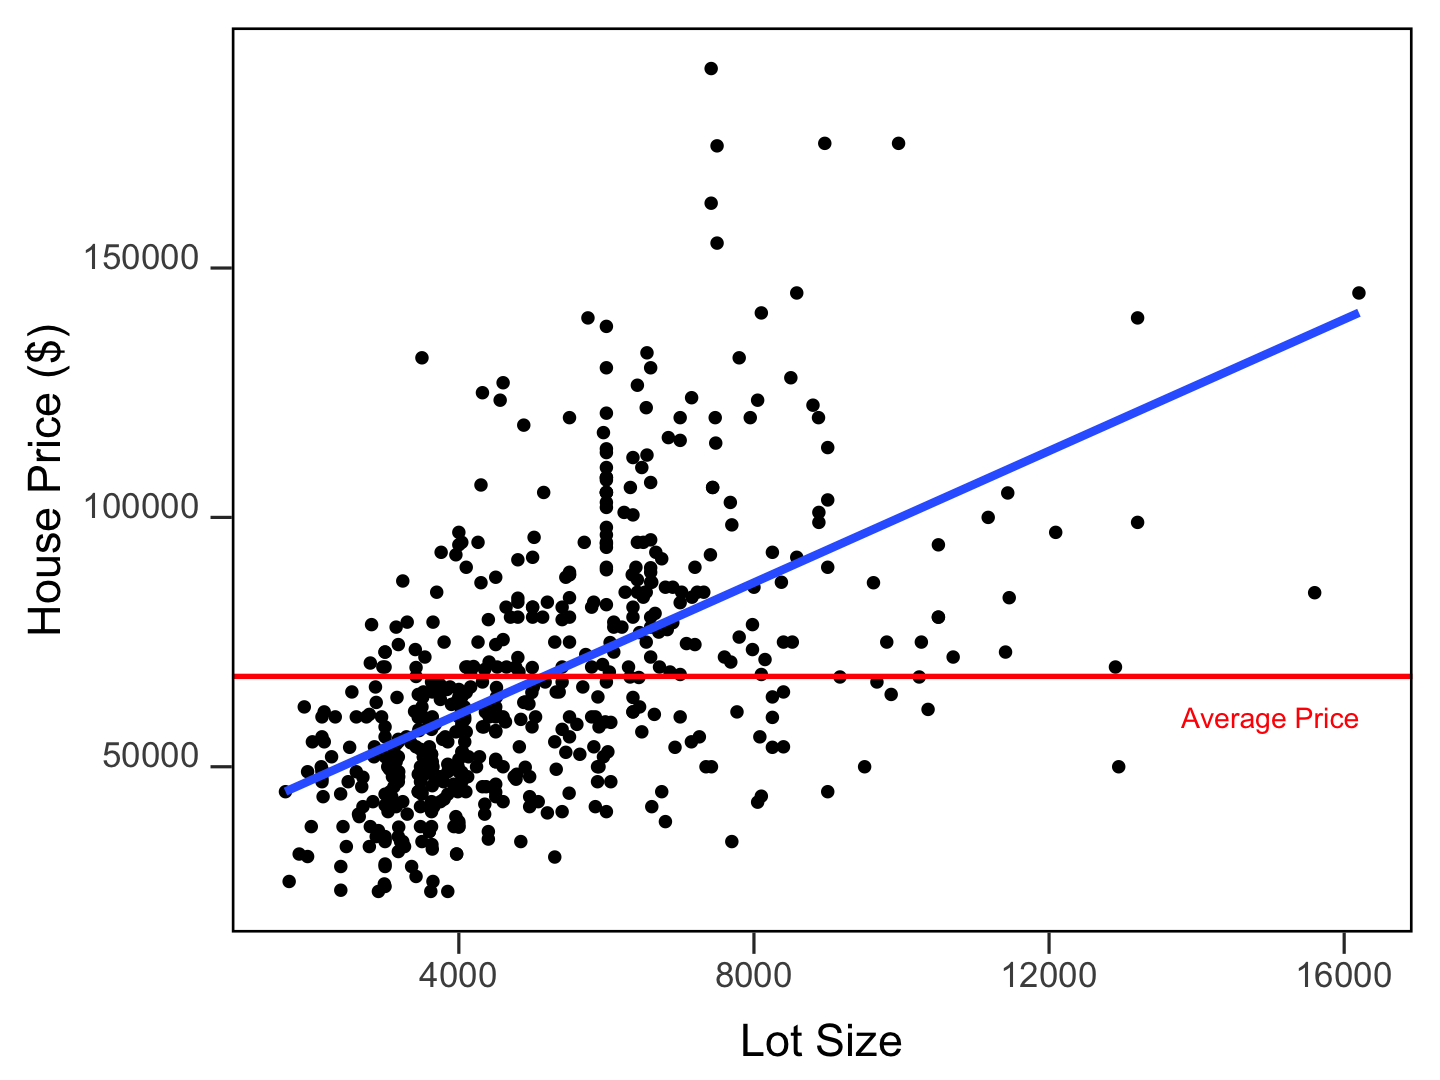
\includegraphics[width=3in,height=3in]{figure/good-1} 

}



\end{knitrout}
  \end{column}
  \begin{column}{0.25\textwidth}
     \begin{itemize}
        \item $y_i-\bar{y}$
        \item $\hat{y_i}-\bar{y}$
        \item $\hat{u_i}$
      \end{itemize}
  \end{column}
​\end{columns}

\end{frame}

\begin{frame}[c]
  \frametitle{$R^2$: Goodness of fit}
  \begin{block}{total sum of squares (SST)}
  \vspace{-0.7cm}
  \begin{align}
     SST\equiv \sum_{i=1}^{n}(y_i-\bar{y})^2 \notag \;\; \mbox{Sample variation in $y$}
  \end{align}
  \end{block}
  \begin{block}{explained sum of squares (SSE)}
  \vspace{-0.7cm}
   \begin{align}
     SSE\equiv \sum_{i=1}^{n}(\hat{y}_i-\bar{y})^2 \notag
  \end{align}
  \end{block}
  \begin{block}{residual sum of squares (SSR)}
  \vspace{-0.7cm}
    \begin{align}
     SSR\equiv \sum_{i=1}^{n}\hat{u}_i^2 \notag
  \end{align}
  \end{block}
\end{frame}

\begin{frame}[c]
  \frametitle{Goodness of fit}
  \begin{block}{$R^2$}
  \vspace{-0.6cm}
     \begin{align}
         R^2 = SSE/SST=1-SSR/SST \notag
     \end{align}
  (the value of $R^2$ always lies between $0$ and $1$ as long as an intercept is included in the econometric model)
  \end{block}
  \begin{block}{What does $R^2$ measure}
    $R^2$ is a measure of how much improvement you've made by including independent variable(s) ($y=\beta_0+\beta_1 x+u$) compared to when simply using the mean of dependent variable as the predictor ($y=\beta_0+u$)
  \end{block}

\end{frame}


\begin{frame}[c]
  \frametitle{$R^2$}
  \begin{block}{Important notes about $R^2$}
    \begin{itemize}
     \item $R^2$ is of no value if you are interested in finding the causal (ceteris paribus) impact of a variable of interest (\textcolor{red}{More on this later when we discuss bias})
     \item $R^2$ is important if your interest lies in predicting $y$
    \end{itemize}
  \end{block}
\end{frame}

%===================================
% Small sample properties
%===================================
\begin{frame}[c]
  \title{Small sample property of OLS estimators}
  \author{}
  \date{}
  \maketitle
\end{frame}

\begin{frame}[c]
  \frametitle{Small sample property of OLS estimators}

  \begin{block}{What is an \textcolor{blue}{estimator}?}
  \begin{itemize}
    \item A function of data that produces an estimate (actual number) of a parameter of interest \textcolor{red}{once} you plug in actual values of data
    \item OLS estimators: $\hat{\beta_1}=\frac{\sum_{i=1}^n(x_i-\bar{x})(y_i-\bar{y})}{\sum_{i=1}^n (x_i-\bar{x})^2}$
  \end{itemize}
  \end{block}

\end{frame}

\begin{frame}[c]
  \frametitle{Small sample property of OLS estimators}

  \begin{block}{What is \textcolor{blue}{small sample property}?}
    Properties that hold whatever the size of observation (small or large) \textcolor{red}{prior to} obtaining actual estimates (before getting data)\\\vspace{0.6cm}

    \begin{itemize}
      \item Put more simply: what can you expect from the estimators before you actually get data and obtain estimates?
      \item Difference between small sample property and the algebraic properties we looked at earlier?
    \end{itemize}
  \end{block}

\end{frame}

\begin{frame}[c]
  \frametitle{Small sample property of OLS estimators}
  \begin{block}{Desirable Properties}
    OLS is only a way of using available information to obtain estimates. Does it have desirable properties?

    \begin{itemize}
      \item Unbiasedness
      \item Efficiency
    \end{itemize}
    \textcolor{blue}{As it turns out, OLS is a very good way of using available information!!}
  \end{block}
\end{frame}

\begin{frame}[c]
  \title{Unbiasedness of OLS estimators}
  \author{}
  \date{}
  \maketitle
\end{frame}

\begin{frame}[c]
  \frametitle{What does \textcolor{blue}{unbiased} mean?}

  \begin{block}{Example}
  \begin{itemize}
    \item Consider a problem of estimating the expected value of a single variable, $x$
    \item A good estimator is sample mean: $\frac{1}{n}\sum_i^n x_i$
  \end{itemize}
  \end{block}
\end{frame}

\begin{frame}[c,fragile]
  \frametitle{Unbiasedness}
  \begin{block_code}{R code: Sample Mean}

  \footnotesize{
\begin{knitrout}
\definecolor{shadecolor}{rgb}{0.969, 0.969, 0.969}\color{fgcolor}\begin{kframe}
\begin{alltt}
\hlcom{#--- set the number of observations ---#}
\hlstd{n} \hlkwb{<-} \hlnum{100}

\hlcom{#--- generate random values ---#}
\hlstd{x_seq} \hlkwb{<-} \hlkwd{rnorm}\hlstd{(n)} \hlcom{# Normal(mean=0,sd=1)}

\hlcom{#--- calcualte the mean ---#}
\hlkwd{mean}\hlstd{(x_seq)}
\end{alltt}
\begin{verbatim}
[1] -0.09058714
\end{verbatim}
\end{kframe}
\end{knitrout}
  }
  \end{block_code}
\end{frame}

\begin{frame}[c,label=unbiased_frame]
  \frametitle{Unbiasedness: Visualization}

\begin{knitrout}
\definecolor{shadecolor}{rgb}{0.969, 0.969, 0.969}\color{fgcolor}

{\centering 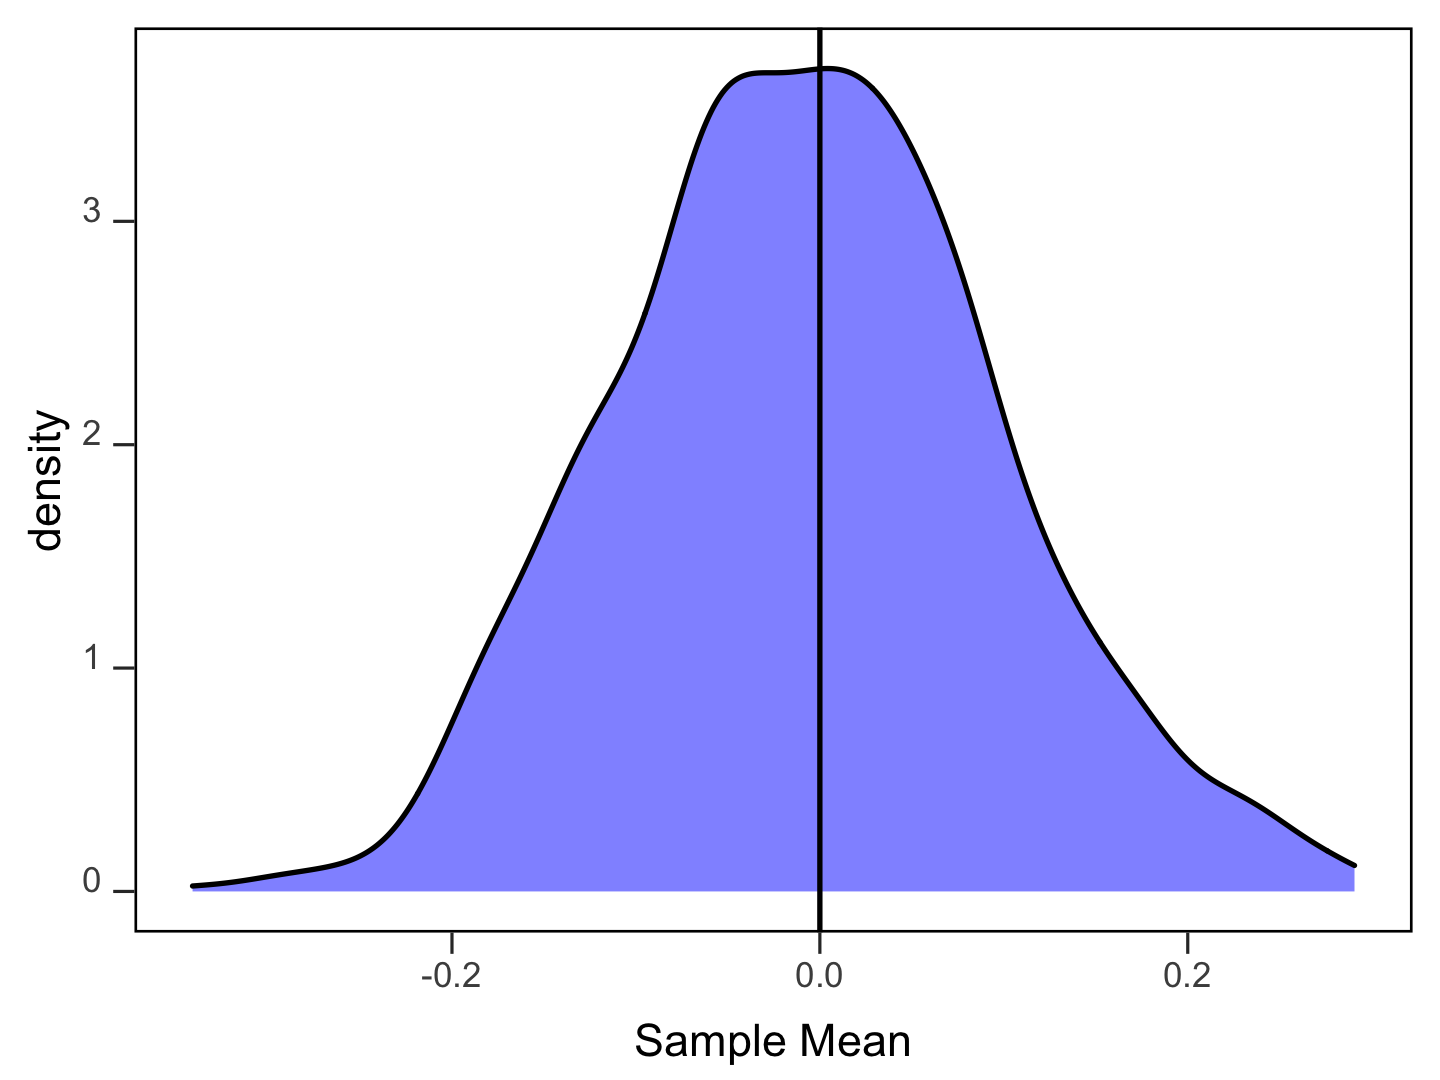
\includegraphics[width=3in,height=3in]{figure/unbiased_viz-1} 

}



\end{knitrout}
\end{frame}

\begin{frame}[c]
  \frametitle{Biasedness: Visualization}

\begin{knitrout}
\definecolor{shadecolor}{rgb}{0.969, 0.969, 0.969}\color{fgcolor}

{\centering 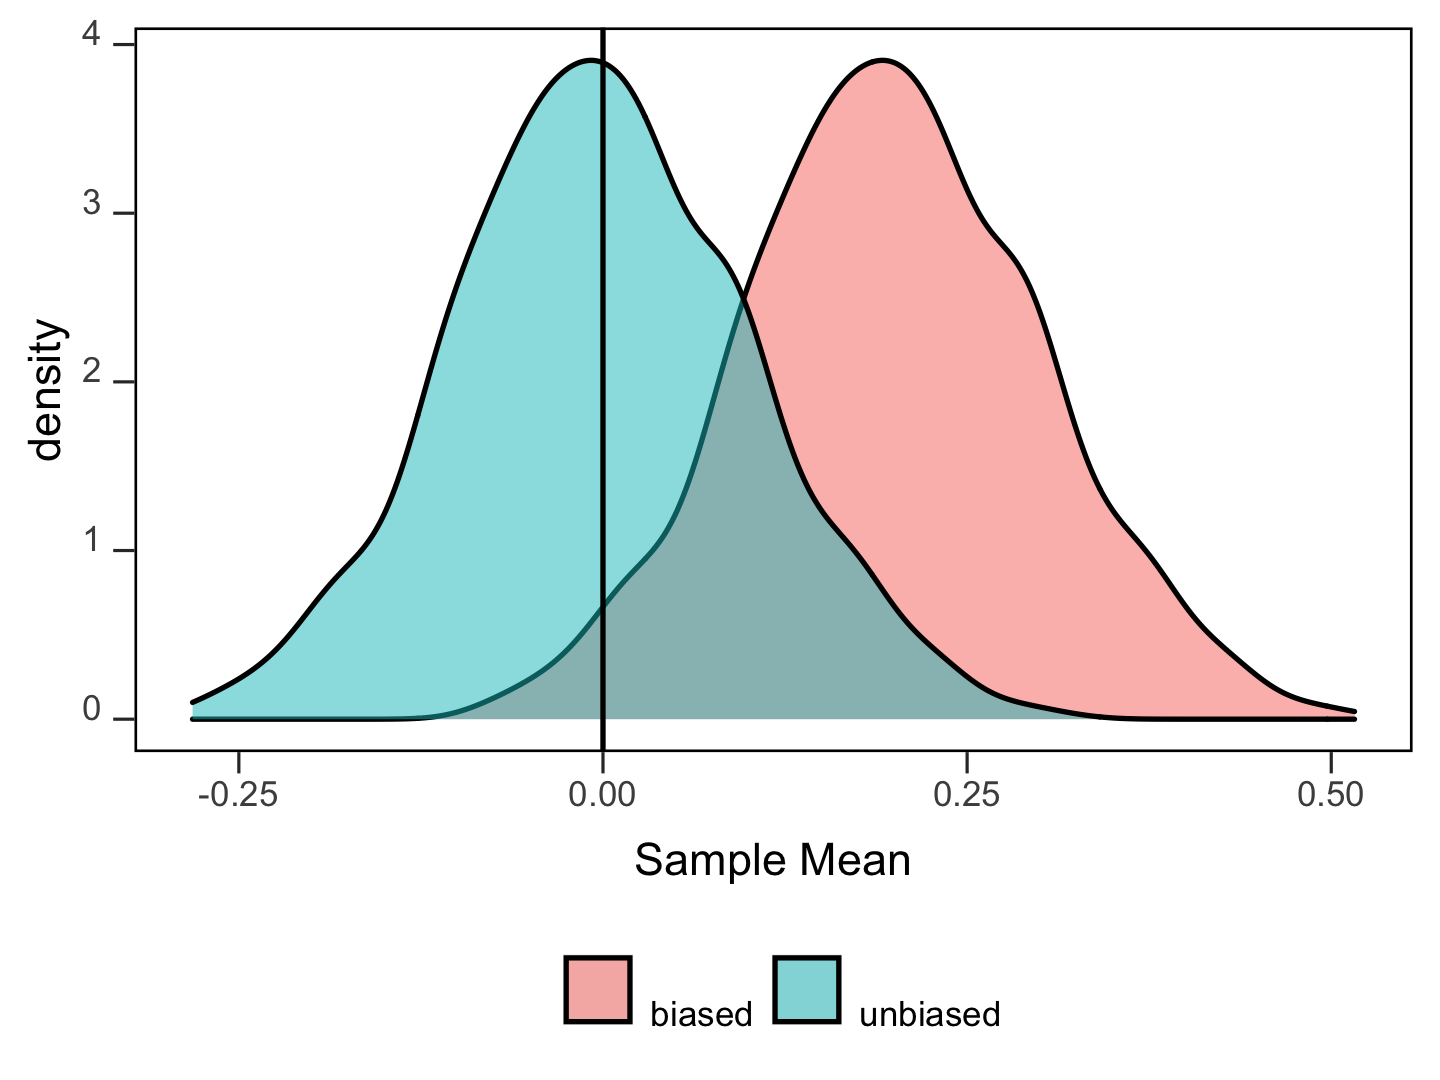
\includegraphics[width=3in,height=3in]{figure/biased_viz-1} 

}



\end{knitrout}
\end{frame}


\begin{frame}[c]
  \frametitle{\textcolor{blue}{Unbiasedness} of OLS estimators}
  \begin{block}{Unbiasedness of OLS estimators}
    Under \textcolor{blue}{certain conditions}, OLS estimators are unbiased. That is,
    \begin{align}
    E[\hat{\beta_1}]=E\Big[\frac{\sum_{i=1}^n(x_i-\bar{x})(y_i-\bar{y})}{\sum_{i=1}^n (x_i-\bar{x})^2}\Big]=\beta_1 \notag
    \end{align}
  \end{block}
  (We do not talk about unbiasedness of $\hat{\beta}_0$ because we are almost never interested in the intercept. Given the limited time we have, it is not worthwhile talking about it)
\end{frame}

\begin{frame}[c]
  \frametitle{Certain Conditions}
  \begin{block}{Condition $SLR.1$: Linear in Parameters}
  In the population model, the dependent variable, $y$, is related to the independent variable, $x$, and the error (or disturbance), $u$, as
  \begin{align*}
         y=\beta_0+\beta_1 x+u \label{peq}
     \end{align*}
  \end{block}
  \tiny{Wooldridge, Jeffrey M. (2012-09-26). Introductory Econometrics: A Modern Approach (Upper Level Economics Titles) (Page 45). Cengage Textbook. Kindle Edition.}
\end{frame}

\begin{frame}[c]
  \frametitle{Certain Conditions}
  \begin{block}{Condition $SLR.2$: Random sampling}
    We have a random sample of size $n$, ${(x_i,y_i):i=1,2,\dots,n}$, following the population model in equation (\ref{peq}). \vspace{0.6cm}

    (\textcolor{blue}{the consequence of the violation of this condition is discussed later})
  \end{block}

  \begin{block}{Non-random sampling}
  \begin{itemize}
    \item Example: You observe income-education data only for those who have income higher than $\$25K$
    \item Benevolent and malevolent kinds:
      \begin{itemize}
        \item \textcolor{blue}{exogenous} sampling
        \item \textcolor{blue}{endogenous} sampling
      \end{itemize}
  \end{itemize}

  \end{block}
  \tiny{Wooldridge, Jeffrey M. (2012-09-26). Introductory Econometrics: A Modern Approach (Upper Level Economics Titles) (Page 45). Cengage Textbook. Kindle Edition.}
\end{frame}

\begin{frame}[c]
  \frametitle{Certain Conditions}
  \begin{block}{Condition $SLR.3$: Sample variation in covariates}
     The sample outcomes on $x$, namely, ${x_i,i=1,\dots,n}$, are not all the same value.
  \end{block}
  \tiny{Wooldridge, Jeffrey M. (2012-09-26). Introductory Econometrics: A Modern Approach (Upper Level Economics Titles) (Page 46). Cengage Textbook. Kindle Edition.}
\end{frame}

\begin{frame}[c]
  \frametitle{Certain Conditions}
  \begin{block}{Condition $SLR.4$: \textcolor{blue}{Zero conditional mean}}
     The error u has an expected value of zero given any value of the explanatory variable. In other words,
  \begin{align}
     E[u|x]=0  \notag
  \end{align}
  Along with random sampling condition, this implies that
  \begin{align}
   E[u_i|x_i]=0 \notag
  \end{align}
  \end{block}
  \tiny{Wooldridge, Jeffrey M. (2012-09-26). Introductory Econometrics: A Modern Approach (Upper Level Economics Titles) (Page 47). Cengage Textbook. Kindle Edition.}
\end{frame}

\begin{frame}[c]
  \frametitle{Correlation and Mean Independence}
  \begin{block}{Note}
    \textcolor{blue}{Mean independence of $u$ and $x$ implies no correlation. But, correlation does not imply mean independence.}
  \end{block}

  \begin{block}{Mean Independence Implies Correlation (Proof)}
  \begin{align*}
     Cov(u,x)= & E[(u-E[u])(x-E[x])] \\
     = & E[ux]-E[u]E[x]-E[u]E[x]+E[u]E[x]\\
     = & E[ux] \\
     = & E_x[E_u[u|x]] \;\; \mbox{(iterated law of expectation)}
  \end{align*}
  If zero conditional mean condition ($E(u|x)=0$) is satisfied,
  \begin{align*}
     Cov(u,x)= & E_x[0] = 0
  \end{align*}
  \end{block}
\end{frame}

\begin{frame}[c]
  \frametitle{Good and bad empiricists}
  \begin{block}{Good Empiricists}
    \begin{itemize}
      \item have ability to judge if the above conditions are satisfied for the particular context you are working on
      \item have ability to correct (if possible) for the problems associated with the violations of any of the above conditions
      \item knows the context well so you can make appropriate judgments
    \end{itemize}
  \end{block}
\end{frame}

\begin{frame}[c]
  \frametitle{Unbiasedness of OLS estimators}
  \begin{align}
    \hat{\beta}_1 = & \frac{\sum_{i=1}^n (x_i-\bar{x})(y_i-\bar{y})}{\sum_{i=1}^n (x_i-\bar{x})^2} \notag \\
    = & \frac{\sum_{i=1}^n (x_i-\bar{x})y_i}{\sum_{i=1}^n (x_i-\bar{x})^2} \;\; \Big[\mbox{because }\sum_{i=1}^n (x_i-\bar{x})\bar{y}=0\Big]\notag\\
    = & \frac{\sum_{i=1}^n (x_i-\bar{x})y_i}{SST_x} \;\;\Big[\mbox{where,}\;\; SST_x=\sum_{i=1}^n (x_i-\bar{x})^2\Big] \notag \\
    = & \frac{\sum_{i=1}^n (x_i-\bar{x})(\beta_0+\beta_1 x_i+u_i)}{SST_x} \notag\\
    = & \frac{\sum_{i=1}^n (x_i-\bar{x})\beta_0 +\sum_{i=1}^n \beta_1(x_i-\bar{x})x_i+\sum_{i=1}^n(x_i-\bar{x})u_i}{SST_x} \notag
  \end{align}
\end{frame}

\begin{frame}[c]
  \frametitle{Unbiasedness of OLS estimators}
  \begin{align*}
    \hat{\beta}_1 = & \frac{\sum_{i=1}^n (x_i-\bar{x})\beta_0 + \beta_1 \sum_{i=1}^n (x_i-\bar{x})x_i+\sum_{i=1}^n(x_i-\bar{x})u_i}{SST_x}
  \end{align*}

  \begin{align*}
    \mbox{Since } & \sum_{i=1}^n (x_i-\bar{x})=0\;\; \mbox{and}\\
     & \sum_{i=1}^n (x_i-\bar{x})x_i=\sum_{i=1}^n (x_i-\bar{x})^2=SST_x,
  \end{align*}

  \begin{align*}
    \hat{\beta}_1 = & \frac{\beta_1 SST_x+\sum_{i=1}^n(x_i-\bar{x})u_i}{SST_x}
    = & \beta_1+(1/SST_x)\sum_{i=1}^n(x_i-\bar{x})u_i
  \end{align*}
\end{frame}

\begin{frame}[c]
  \frametitle{Unbiasedness of OLS estimators}
 \begin{align}
    \hat{\beta}_1 = & \beta_1+(1/SST_x)\sum_{i=1}^n(x_i-\bar{x})u_i \notag
 \end{align}
 Taking, expectation of $\hat{\beta}_1$ conditional on $\mathbf{x}=\{x_1,\dots,x_n\}$,
 \begin{align}
    \Rightarrow E[\hat{\beta}_1|\mathbf{x}] = & E[\beta_1|\mathbf{x}]+E[(1/SST_x)\sum_{i=1}^n(x_i-\bar{x})u_i|\mathbf{x}] \notag \\
    = & \beta_1 + (1/SST_x)\sum_{i=1}^n (x_i-\bar{x}) E[u_i|\mathbf{x}] \notag
 \end{align}

 So, if condition 4 ($E[u_i|\mathbf{x}]=0$) is satisfied,
 \begin{align}
    E[\hat{\beta}_1|\mathbf{x}] = & \beta_1 \notag\\
    E_{\mathbf{x}}[\hat{\beta}_1|\mathbf{x}] = & E[\hat{\beta}_1] = \beta_1 \notag
 \end{align}
\end{frame}

\begin{frame}[c]
  \frametitle{Unbiasedness of OLS estimators}

  \begin{block}{Reconsider the following example}
  \vspace{-0.6cm}
   \begin{align}
    price=\beta_0+\beta_1\times lotsize + u \notag
  \end{align}
  \vspace{-0.6cm}
  \begin{itemize}
    \item $price$: house price (\$)
    \item $lotsize$: lot size
    \item $u$: error term (everything else)
  \end{itemize}
  \end{block}

  \begin{block}{Questions}
    \begin{itemize}
       \item What's in $u$?
       \item Do you think $E[u|x]$ is satisfied?
     \end{itemize}
  \end{block}
\end{frame}

\begin{frame}[c]
  \frametitle{Unbiasedness of OLS estimators}
  \begin{block}{Important notes (again)}
  \begin{itemize}
    \item Unbiasedness property of OLS estimators says \textcolor{blue}{NOTHING} about the estimate that we obtain for a given sample
    \item it is always possible that we could obtain an unlucky sample that would give us a point estimate far from $\beta_1$, and we can never know for sure whether this is the case.
  \end{itemize}
  \end{block}
\end{frame}

\begin{frame}[c]
  \title{Variance of OLS estimators}
  \author{}
  \date{}
  \maketitle
\end{frame}

\begin{frame}[c]
  \frametitle{Variance of OLS estimators}
  \begin{block}{Important notes}
    \begin{itemize}
      \item OLS estimators are random variables, which means that they have distributions
      \item OLS estimators have variance (how spread out OLS estimates can be)
    \end{itemize}
  \end{block}
\end{frame}

\begin{frame}[c]
  \frametitle{Variance}
  \begin{block}{Example:}
    Consider two estimators of $E[x]$:
    \begin{align}
      \theta_{smart} = & \frac{1}{n}\sum_{i=1}^n x_i  \;\;(n=1000)\notag \\
      \theta_{stupid} = & \frac{1}{10}\sum_{i=1}^{10} x_i \notag
    \end{align}
  \end{block}
\end{frame}

\begin{frame}[c,label=var_frame]
  \frametitle{Variance of estimators}
\begin{knitrout}
\definecolor{shadecolor}{rgb}{0.969, 0.969, 0.969}\color{fgcolor}

{\centering 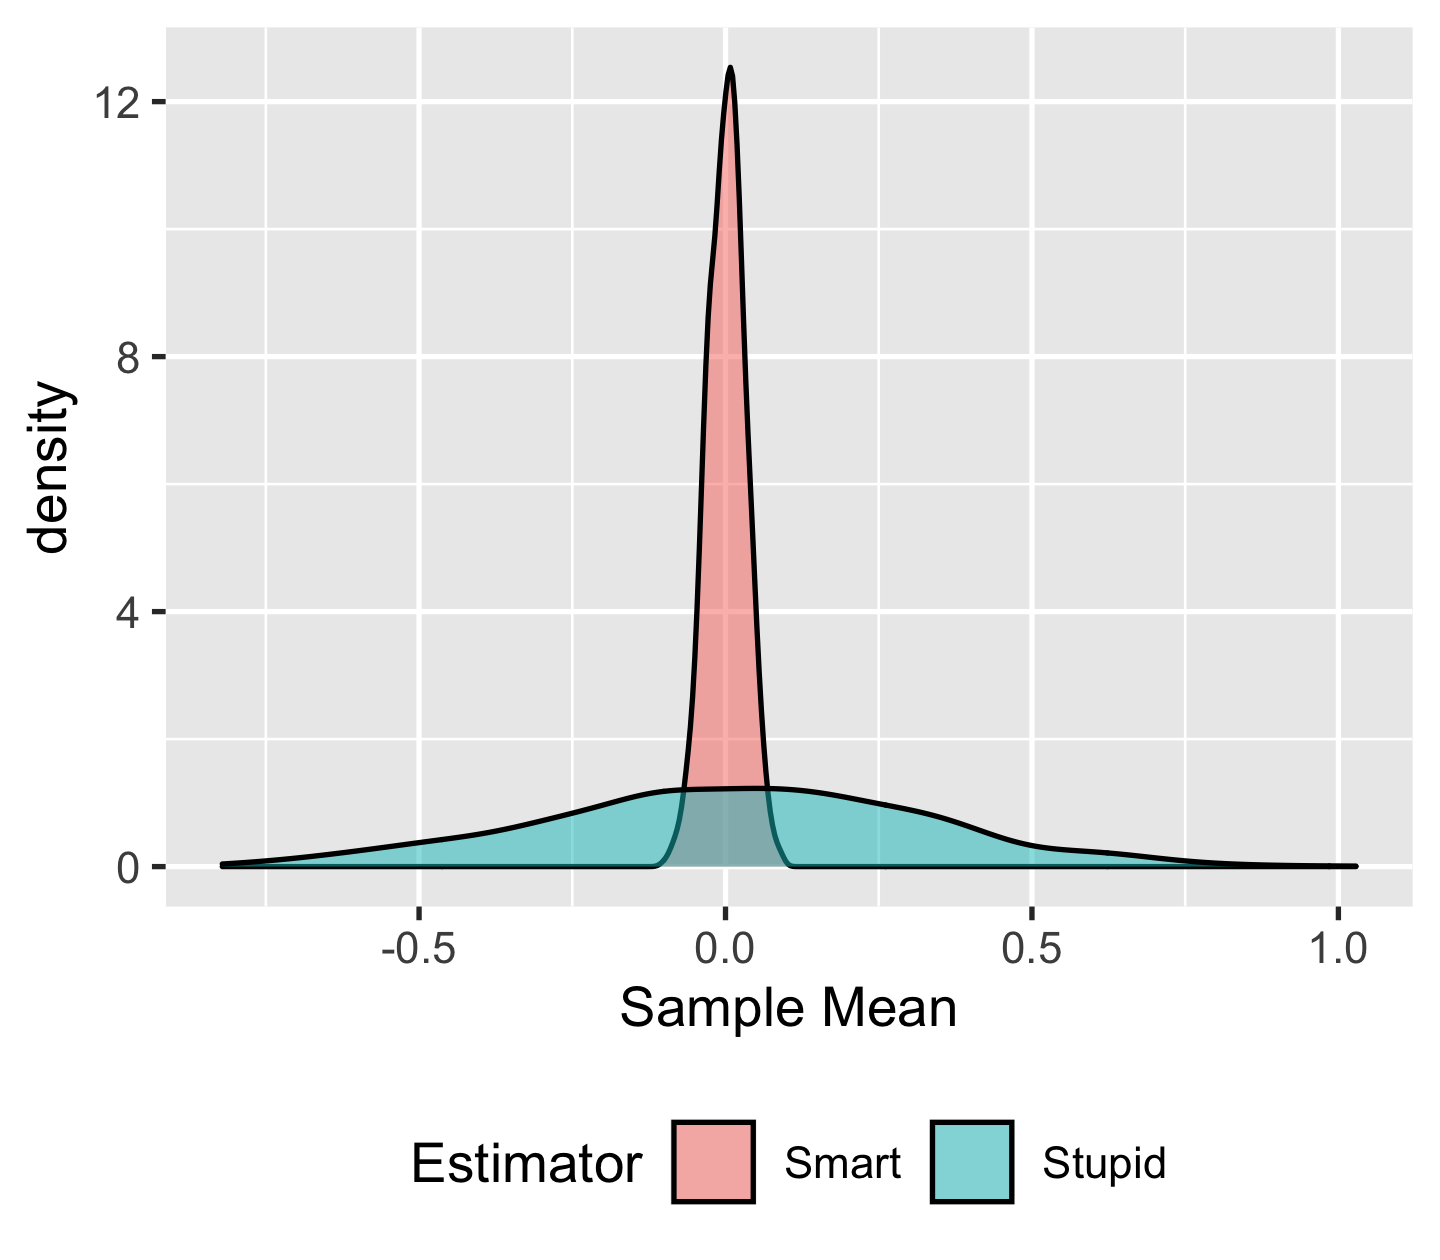
\includegraphics[width=3in,height=3in]{figure/variance_viz-1} 

}



\end{knitrout}
\end{frame}

\begin{frame}[c]
  \frametitle{Variance of OLS estimators}

  \begin{block}{Variance of OLS estimators}
  If \textcolor{blue}{$Var(u|x)=\sigma^2$} and the four conditions (we used to prove unbiasedness of OLS estimators) are satisfied,
    \begin{align}
      Var(\hat{\beta}_1) = \frac{\sigma^2}{\sum_{i=1}^n (x_i-\bar{x})^2}=\frac{\sigma^2}{SST_x} \notag
    \end{align}
  \end{block}
\end{frame}

\begin{frame}[c]
  \frametitle{$Var(u|x)=\sigma^2$}
  \begin{block}{Homoskedasticity}
    The error $u$ has the same variance give any value of the covariate $x$
  \end{block}

  \begin{block}{Heterokedasticity}
    The variance of the error $u$ differs depending on the value of $x$
    \begin{align}
       Var(u|x)=f(x)
    \end{align}
  \end{block}
\end{frame}



\begin{frame}[c]
  \frametitle{Homoskedastic Error}
\begin{knitrout}
\definecolor{shadecolor}{rgb}{0.969, 0.969, 0.969}\color{fgcolor}

{\centering \includegraphics[width=3in,height=3in]{figure/fig_homoske-1} 

}



\end{knitrout}
\end{frame}

\begin{frame}[c]
  \frametitle{Heteroskedastic Error}
\begin{knitrout}
\definecolor{shadecolor}{rgb}{0.969, 0.969, 0.969}\color{fgcolor}

{\centering \includegraphics[width=3in,height=3in]{figure/fig_hetero-1} 

}



\end{knitrout}
\end{frame}

\begin{frame}[c]
  \frametitle{House Price Example}

\begin{knitrout}
\definecolor{shadecolor}{rgb}{0.969, 0.969, 0.969}\color{fgcolor}

{\centering \includegraphics[width=3in,height=3in]{figure/price_hetero-1} 

}



\end{knitrout}
\end{frame}

\begin{frame}[c]
  \frametitle{Homoskedasticity Condition (Assumption)}
  \begin{block}{Important notes}
    \begin{itemize}
      \item We did \textcolor{blue}{NOT} use this condition to prove that OLS estimators are unbiased
      \item In most applications, homoskedasticity condition is not satisfied, which has important implications on:
        \begin{itemize}
          \item estimation of variance (standard error) of OLS estimators
          \item significance test
        \end{itemize}
      (\textcolor{red}{A lot more on this issue later})
    \end{itemize}
  \end{block}
\end{frame}

\begin{frame}[c,label=var_dev]
  \frametitle{Derivation of the variance of OLS estimators}

  \begin{align}
    \hat{\beta}_1 = & \beta_1 + (1/SST_x)\sum_{i=1}^n d_i u_i \notag
  \end{align}
  Because $Var(\alpha x)=\alpha^2 var(x)$,
  \begin{align}
    Var(\hat{\beta}_1|x) = & (1/SST_x)^2 Var(\sum_{i=1}^n d_i u_i|x) \notag
  \end{align}
  Because of independent random sampling \hyperlink{mathasides}{\beamerbutton{Math Aside}},
  \begin{align}
    Var(\hat{\beta}_1|x) = & (1/SST_x)^2 \sum_{i=1}^n d_i^2 Var(u_i|x) \notag
  \end{align}
  If the homoskedasticity assumption is satisfied,
  \begin{align}
    Var(\hat{\beta}_1|x) = & (1/SST_x)^2 \sum_{i=1}^n d_i^2 \sigma^2 \notag \\
    = & \sigma^2/SST_x \notag
  \end{align}
\end{frame}

\begin{frame}[c,label=mathasides]
  \frametitle{Math Aside \hyperlink{var_dev}{\beamerbutton{Go Back}}}
  \begin{align}
    Var(\alpha x) = & \alpha^2 Var(x)\notag \\
    Var(x+y) = & Var(x) + 2Cov(x,y) + Var(y)\notag
  \end{align}
  If $x$ and $y$ are independent, $Cov(x,y) =0$.
\end{frame}

\begin{frame}[c]
  \frametitle{Variance of OLS estimators}
  \begin{block}{Variance of the OLS estimators}
  \vspace{-0.6cm}
    \begin{align*}
    Var(\hat{\beta}_1|x) = \sigma^2/SST_x \notag
    \end{align*}
  \end{block}
  \only<2->{\begin{block}{What can you learn from this equation?}
     \begin{itemize}
    \item the variance of OLS estimators is smaller (larger) if the variance of error term is smaller (larger)
    \item the greater (smaller) the variation in the covariate $x$, the smaller (larger) the variance of OLS estimators
      \begin{itemize}
        \item if you are running experiments, spread the value of $x$ as much as possible
        \item you will rarely have this luxury
      \end{itemize}
    \end{itemize}
   \end{block}}
\end{frame}

\begin{frame}[c]
  \frametitle{Gauss-Markov Theorem:}
  \begin{block}{Gauss-Markov Theorem}
    Under conditions $SLR.1$ through $SLR.5$, OLS estimators are the best linear unbiased estimators (BLUEs)
  \end{block}
  \begin{block}{Meaning,}
    No other \textcolor{blue}{unbiased linear}  estimators have smaller variance than the OLS estimators (desirable efficiency property of OLS)
  \end{block}
\end{frame}

\begin{frame}[c]
  \frametitle{Estimating the error variance}

  \begin{itemize}
    \item $Var(\hat{\beta}_1|x) = \sigma^2/SST_x$ will never be known. But, you can estimate it.
    \item Once you estimate $Var(\hat{\beta}_1|x)$, you can test the statistical significance of $\hat{\beta}_1$ (More on this later)
  \end{itemize}
\end{frame}

\begin{frame}[c]
  \frametitle{Estimating the error variance}
  \begin{align}
    & Var(u_i)=\sigma^2=E[u_i^2] \notag \\
    & \Big( Var(u_i)\equiv E[u_i^2]-E[u_i]^2 \Big) \notag
  \end{align}
  \begin{itemize}
    \item So, $\frac{1}{n}\sum_{i=1}^n u_i^2$ is an unbiased estimator of $Var(u_i)$
    \item What is the problem with this estimator?
  \end{itemize}
\end{frame}

\begin{frame}[c]
  \frametitle{Estimating the error variance}
  We don't observe $u_i$ (error), but we observe residuals ($\hat{u_i}$)
  \begin{block}{Error and Residual}
  \vspace{-0.6cm}
    \begin{align}
       y_i = \beta_0+\beta_1 x_i + u_i \notag\\
       y_i = \hat{\beta}_0+\hat{\beta}_1 x_i + \hat{u}_i \notag
    \end{align}
  \end{block}

  \begin{block}{Residuals as unbiased estimators of error}
  \vspace{-0.6cm}
   \begin{align}
      \hat{u}_i = & y_i -\hat{\beta}_0-\hat{\beta}_1 x_i \notag\\
      \hat{u}_i = & \beta_0+\beta_1 x_i + u_i -\hat{\beta}_0-\hat{\beta}_1 x_i \notag\\
      \Rightarrow \hat{u}_i -u_i=&(\beta_0-\hat{\beta}_0)+(\beta_1-\hat{\beta}_1) x_i \notag\\
      \Rightarrow E[\hat{u}_i -u_i]=&E[(\beta_0-\hat{\beta}_0)+(\beta_1-\hat{\beta}_1) x_i]=0\notag
  \end{align}
  \end{block}
\end{frame}

\begin{frame}[c]
  \frametitle{Estimating the error variance}
  \begin{itemize}
    \item We know $E[\hat{u}_i-u_i]=0$
    \item so, why don't we use $\hat{u}_i$ (observable) in place of $u_i$ (unobservable)
    \item $\frac{1}{n}\sum_{i=1}^n \hat{u}_i^2$ as an estimator of $\sigma^2$?
    \item Unfortunately, $\frac{1}{n}\sum_{i=1}^n \hat{u}_i^2$ is a biased estimator of $\sigma^2$
  \end{itemize}
\end{frame}

\begin{frame}[c]
  \frametitle{Estimating the error variance}
   \begin{block}{Algebraic property of OLS}
  \vspace{-0.6cm}
    \begin{align}
        \sum_{i=1}^n \hat{u}_i=0\;\; \mbox{and}\;\; \sum_{i=1}^n x_i\hat{u}_i=0\notag
    \end{align}
  \only<2->{\begin{itemize}
    \item this means that once you know the value of $n-2$ residuals, you can find the value of the other two by solving the above equations
    \item so, it's almost as if you have $n-2$ value of residuals instead of $n$
  \end{itemize}}
  \end{block}
  \only<3->{\begin{block}{Unbiased estimator of $\sigma^2$}
    We use $\hat{\sigma}^2=\frac{1}{n-2}\sum_{i=1}^n \hat{u}_i^2$, which satisfies $E[\frac{1}{n-2}\sum_{i=1}^n \hat{u}_i^2]=\sigma^2$
  \end{block}}
\end{frame}

\begin{frame}[c]
  \frametitle{The use of $\hat{\sigma}^2$}
  Since $sd(\hat{\beta_1})=\sigma/\sqrt{SST_x}$, the natural estimator of $sd(\hat{\beta_1})$ is
  \begin{align*}
     se(\hat{\beta_1}) =\sqrt{\hat{\sigma}^2}/\sqrt{SST_x},
  \end{align*}
  which is called \textcolor{blue}{standard error of $\hat{\beta_1}$}. Later, we use $\hat{\beta_1}$ for testing.
\end{frame}

\begin{frame}[c,fragile]
  \frametitle{Standard Error Estimation}

  \begin{block_code}{R code: Standard Error}
  \scriptsize{
\begin{knitrout}
\definecolor{shadecolor}{rgb}{0.969, 0.969, 0.969}\color{fgcolor}\begin{kframe}
\begin{alltt}
\hlkwd{summary}\hlstd{(uni_reg)}
\end{alltt}
\begin{verbatim}

Call:
lm(formula = price ~ lotsize, data = HousePrices)

Residuals:
   Min     1Q Median     3Q    Max 
-69551 -14626  -2858   9752 106901 

Coefficients:
             Estimate Std. Error t value Pr(>|t|)    
(Intercept) 3.414e+04  2.491e+03    13.7   <2e-16 ***
lotsize     6.599e+00  4.458e-01    14.8   <2e-16 ***
---
Signif. codes:  0 '***' 0.001 '**' 0.01 '*' 0.05 '.' 0.1 ' ' 1

Residual standard error: 22570 on 544 degrees of freedom
Multiple R-squared:  0.2871,	Adjusted R-squared:  0.2858 
F-statistic: 219.1 on 1 and 544 DF,  p-value: < 2.2e-16
\end{verbatim}
\end{kframe}
\end{knitrout}
  }
  \end{block_code}
\end{frame}

%===================================
% functional form and scale
%===================================


\begin{frame}[c]
  \title{Functional Form}
  \author{}
  \date{}
  \maketitle
\end{frame}

\begin{frame}[c]
  \frametitle{Functional Form}
  \begin{block}{Functional forms}
    \begin{itemize}
    \item transformation of variables is allowed without disturbing our analytical framework as long as the model is linear in \textcolor{blue}{parameter}.
    \item transformation of variables change the interpretation of the coefficients estimates
    \end{itemize}
  \end{block}
  \begin{block}{Golas}
    \begin{itemize}
      \item present popular functional forms
      \item use simple calculus to examine the interpretation of the coefficients
    \end{itemize}
  \end{block}
\end{frame}

\begin{frame}[c]
  \frametitle{Popular Functional Forms}
  \begin{block}{log-linear}
  \vspace{-0.6cm}
    \begin{align}
     log(y_i)= \beta_0+\beta_1 x_i + u_i \notag
    \end{align}
  \end{block}
  \begin{block}{linear-log}
  \vspace{-0.6cm}
    \begin{align}
     y_i= \beta_0+\beta_1 log(x_i) + u_i \notag
    \end{align}
  \end{block}
  \begin{block}{log-log}
  \vspace{-0.6cm}
    \begin{align}
     log(y_i)= \beta_0+\beta_1 log(x_i) + u_i \notag
    \end{align}
  \end{block}
\end{frame}

\begin{frame}[c]
  \frametitle{Functional form: Log-linear}
  \begin{block}{Model}
  \vspace{-0.6cm}
    \begin{align}
      log(y_i)= \beta_0+\beta_1 x_i + u_i \notag
    \end{align}
  \end{block}

  \begin{block}{Calculus}
    Differentiating the both sides wrt $x_i$,
    \begin{align}
      \frac{1}{y_i}\cdot\frac{\partial y_i}{\partial x_i} = \beta_1 \Rightarrow \frac{\Delta y_i}{y_i} = \beta_1 \Delta x_i \notag
    \end{align}
  \end{block}

  \begin{block}{Interpretation}
    $\beta_1$ measures a percentage change in $y_i$ when $x_i$ is increased by one unit
  \end{block}
\end{frame}




% \begin{frame}[c]
%   \frametitle{Functional Form}
% \begin{columns}[onlytextwidth]
%   \begin{column}{0.55\textwidth}
% <<g_wage_2, echo=FALSE,out.height='2.1in',out.width='2.1in',dev='pdf'>>=
% g_wage_loess
% @
%   \end{column}
%   \begin{column}{0.45\textwidth}
%     So far, $y$ and $x$ are linearly related in all the models we have considered\\ \vspace{0.6cm}
%     $\hat{wage}=-0.90+0.54\times educ$
%   \end{column}
% ​\end{columns}
% \end{frame}

\begin{frame}[c]
  \frametitle{Functional Form}
  It is not hard to write the model in a way that $y$ and $x$ are non-linearly related. \vspace{0.6cm}

  How about this model?
  \begin{align}
     log(wage)=\beta_0 + \beta_1 educ + u \notag
  \end{align}

  Interpretation of $\beta_1$? Differentiating both sides with respect to $educ$,
  \begin{align}
     \frac{1}{wage} \frac{\partial wage}{\partial educ} = \beta_1 \Rightarrow \frac{\Delta wage}{wage} = \beta_1\Delta educ\notag
  \end{align}
  \begin{block}{Interpretation}
    If education increases by 1 year ($\Delta educ=1$), then wage increases by $\beta_1*100\%$ ($\frac{\Delta wage}{wage}=\beta_1$)
  \end{block}
\end{frame}

\begin{frame}[c]
  \frametitle{Log-linear model}
  If you estimate $log(wage)=\beta_0 + \beta_1 educ + u \notag$,
  \begin{align}
    \widehat{log(wage)}=0.584+0.083 educ \notag
  \end{align}
  With $u=0$,
  \begin{align}
    \widehat{wage}=e^{0.584+0.083 educ} \notag
  \end{align}
\end{frame}

\begin{frame}[c]
  \frametitle{Visualization}
\begin{knitrout}
\definecolor{shadecolor}{rgb}{0.969, 0.969, 0.969}\color{fgcolor}

{\centering 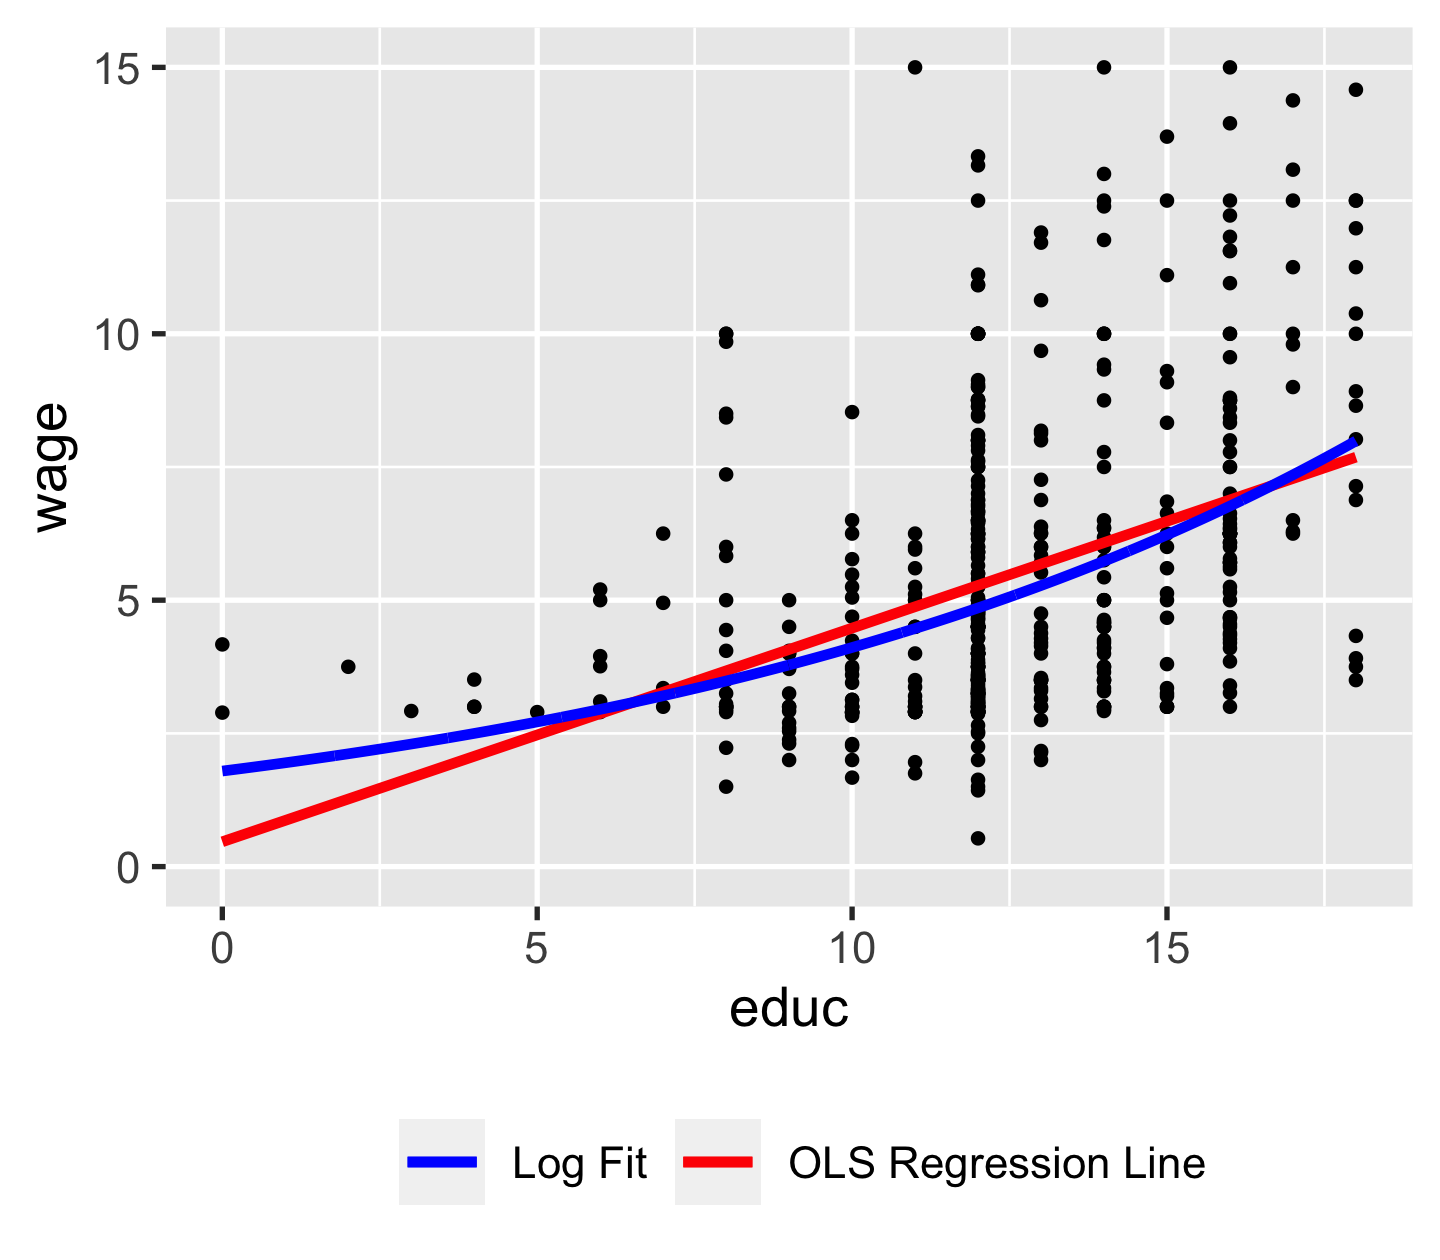
\includegraphics[width=3in,height=3in]{figure/g_wage_log-1} 

}



\end{knitrout}
\end{frame}


% \begin{frame}[c,fragile]
%   \frametitle{Visualization}
%   \begin{figure}
%   \caption[]{Visualization of log-linear functional form: $E[y|x]=exp(\beta_0+\beta_1 x)$}
%   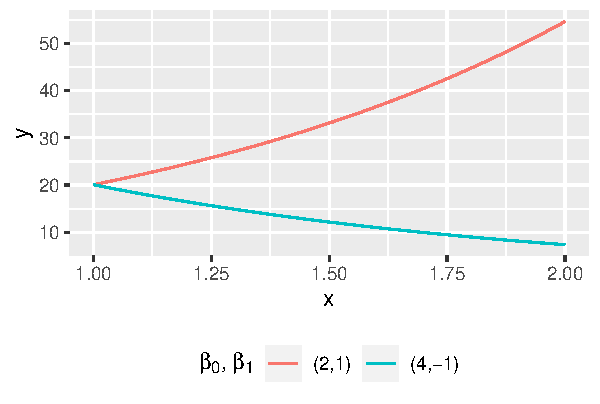
\includegraphics[width=4in]{log_linear_vis.pdf}
%   \end{figure}
% \end{frame}

\begin{frame}[c]
  \frametitle{Functional form: Linear-log}
  \begin{block}{Model}
    \begin{align}
      y_i= \beta_0+\beta_1 log(x_i) +u_i \notag
    \end{align}
  \end{block}

  \begin{block}{Calculus}
    Differentiating the both sides wrt $x_i$,
    \begin{align}
      \frac{\partial y_i}{\partial x_i} = \beta_1/x_i \Rightarrow \Delta y_i = \beta_1\frac{\Delta x_i}{x_i} \notag
    \end{align}
  \end{block}
  \begin{block}{Interpretation}
    When $x$ increases by $1\%$, $y$ increases by $\beta_1$
  \end{block}
\end{frame}

\begin{frame}[c,fragile]
  \frametitle{Visualization}
\begin{knitrout}
\definecolor{shadecolor}{rgb}{0.969, 0.969, 0.969}\color{fgcolor}

{\centering 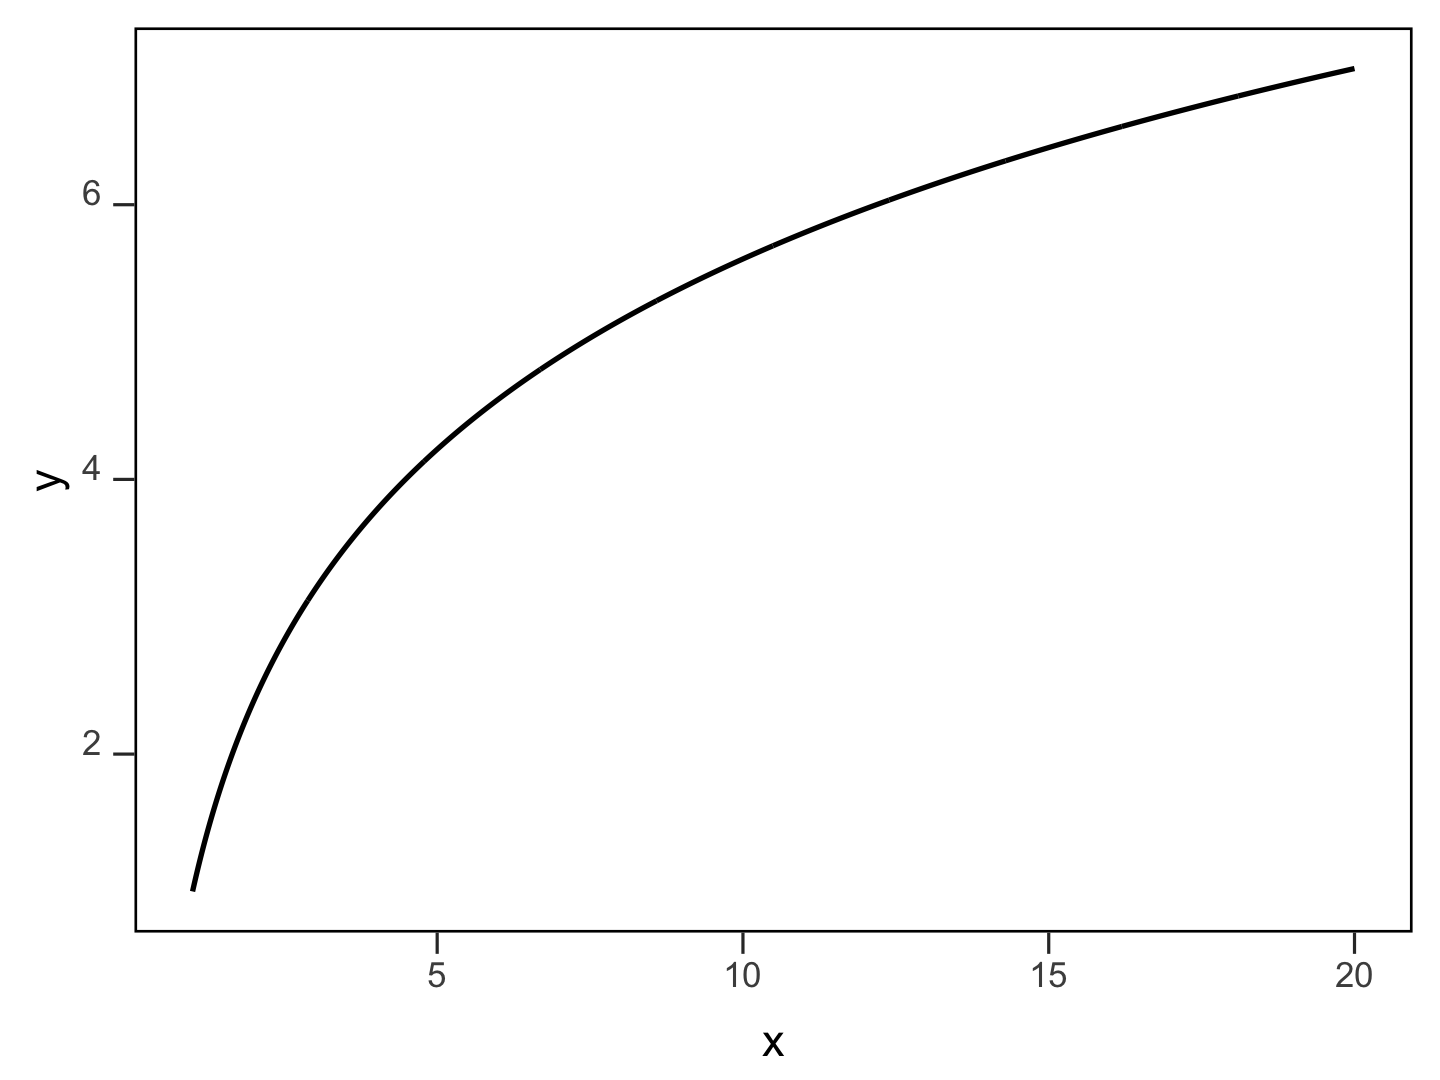
\includegraphics[width=3in,height=3in]{figure/linear_log_vis-1} 

}



\end{knitrout}
\end{frame}


\begin{frame}[c]
  \frametitle{Functional form: Log-log}
  \begin{block}{model}
  \vspace{-0.6cm}
    \begin{align}
    log(y_i)= \beta_0+\beta_1 log(x_i) +u_i \notag
  \end{align}
  \end{block}

  \begin{block}{Calculus}
    Differentiating the both sides wrt $x_i$,
    \begin{align}
      \frac{\partial y_i}{y_i}/\frac{\partial x_i}{x_i} = \beta_1 \Rightarrow \frac{\Delta y_i}{y_i} = \beta_1 \frac{\Delta x_i}{x_i}\notag
    \end{align}
  \end{block}

  \begin{block}{Interpretation}
    A \textcolor{blue}{percentage} change in $x$ would result in a $\beta_1$ \textcolor{blue}{percentage} change in $y_i$ (constant elasticity)
  \end{block}
\end{frame}


\begin{frame}[c]
  \frametitle{Simple Linear Regression}
  \begin{itemize}
    \item In these models, the dependent variable and independent variable are non-linearly related, how come are these models called simple \textcolor{blue}{linear} model?
    \item \textcolor{blue}{``linear''} in simple \textcolor{blue}{linear} model means that the model is linear in \textcolor{blue}{parameter}, but not in \textcolor{blue}{variable}
  \end{itemize}

\end{frame}

\begin{frame}[c]
  \frametitle{Non-linear (in parameter) Models}
  \begin{block}{Examples: non-linear models}
  \vspace{-0.6cm}
    \begin{align*}
      y_i=\beta_0+x_i^{\beta_1}+u_i \\
      y_i=\frac{x_i}{\beta_0+\beta_1 x_i}+u_i
    \end{align*}
  \end{block}
  \begin{block}{Notes}
    Transformation of the dependent and independent variables would not affect the OLS results we have seen as long as the model is linear in parameter
  \end{block}
\end{frame}

%===================================
% Appendix
%===================================
\appendix
\title{Appendix}
\author{}
\date{}

\begin{frame}[c]
\maketitle
\end{frame}

\begin{frame}[c,fragile,label=R_unbiased]
  \frametitle{R code to generate the unbiasedness figure \hyperlink{unbiased_frame}{\beamerbutton{go back}}}
 \scriptsize{
\begin{knitrout}
\definecolor{shadecolor}{rgb}{0.969, 0.969, 0.969}\color{fgcolor}\begin{kframe}
\begin{alltt}
  \hlcom{#--- set seed ---#}
  \hlkwd{set.seed}\hlstd{(}\hlnum{244598}\hlstd{)}

  \hlcom{#--- set the number of observations ---#}
  \hlstd{n} \hlkwb{<-} \hlnum{100}
  \hlstd{B} \hlkwb{<-} \hlnum{1000}
  \hlstd{mean_st} \hlkwb{<-} \hlkwd{rep}\hlstd{(}\hlnum{0}\hlstd{,B)}
  \hlkwa{for} \hlstd{(i} \hlkwa{in} \hlnum{1}\hlopt{:}\hlstd{B)\{}
    \hlcom{#--- generate random values ---#}
    \hlstd{x_seq} \hlkwb{<-} \hlkwd{rnorm}\hlstd{(n)} \hlcom{# Normal(mean=0,sd=1)}

    \hlcom{#--- calcualte the mean ---#}
    \hlstd{mean_st[i]} \hlkwb{<-} \hlkwd{mean}\hlstd{(x_seq)}
  \hlstd{\}}
  \hlstd{plot_data} \hlkwb{<-} \hlkwd{data.table}\hlstd{(mean_st)}
  \hlstd{g_unsbiased} \hlkwb{<-} \hlkwd{ggplot}\hlstd{(}\hlkwc{data}\hlstd{=plot_data)} \hlopt{+}
    \hlkwd{geom_density}\hlstd{(}\hlkwd{aes}\hlstd{(}\hlkwc{x}\hlstd{=mean_st),}\hlkwc{fill}\hlstd{=}\hlstr{'blue'}\hlstd{,}\hlkwc{alpha}\hlstd{=}\hlnum{0.5}\hlstd{)} \hlopt{+}
    \hlkwd{xlab}\hlstd{(}\hlstr{'Sample Mean'}\hlstd{)}
\end{alltt}
\end{kframe}
\end{knitrout}
}
\end{frame}

\begin{frame}[c,fragile,label=R_var]
  \frametitle{R code to generate the variance figure \hyperlink{var_frame}{\beamerbutton{go back}}}
 \scriptsize{
\begin{knitrout}
\definecolor{shadecolor}{rgb}{0.969, 0.969, 0.969}\color{fgcolor}\begin{kframe}
\begin{alltt}
  \hlkwd{set.seed}\hlstd{(}\hlnum{38495}\hlstd{)}
  \hlstd{B} \hlkwb{<-} \hlnum{1000}
  \hlstd{theta_smart} \hlkwb{<-} \hlkwd{rep}\hlstd{(}\hlnum{0}\hlstd{,B)}
  \hlstd{theta_stupid} \hlkwb{<-} \hlkwd{rep}\hlstd{(}\hlnum{0}\hlstd{,B)}
  \hlkwa{for} \hlstd{(i} \hlkwa{in} \hlnum{1}\hlopt{:}\hlstd{B)\{}
    \hlstd{x} \hlkwb{<-} \hlkwd{rnorm}\hlstd{(}\hlnum{1000}\hlstd{)}
    \hlstd{theta_smart[i]} \hlkwb{<-} \hlkwd{mean}\hlstd{(x)}
    \hlstd{theta_stupid[i]} \hlkwb{<-} \hlkwd{mean}\hlstd{(x[}\hlnum{1}\hlopt{:}\hlnum{10}\hlstd{])}
  \hlstd{\}}

  \hlstd{smart_data} \hlkwb{<-} \hlkwd{data.table}\hlstd{(}\hlkwc{value}\hlstd{=theta_smart,}\hlkwc{type}\hlstd{=}\hlstr{'Smart'}\hlstd{)}
  \hlstd{stupid_data} \hlkwb{<-} \hlkwd{data.table}\hlstd{(}\hlkwc{value}\hlstd{=theta_stupid,}\hlkwc{type}\hlstd{=}\hlstr{'Stupid'}\hlstd{)}
  \hlstd{plot_data} \hlkwb{<-} \hlkwd{rbind}\hlstd{(smart_data,stupid_data)}

  \hlstd{g_var} \hlkwb{<-} \hlkwd{ggplot}\hlstd{(}\hlkwc{data}\hlstd{=plot_data)} \hlopt{+}
    \hlkwd{geom_density}\hlstd{(}\hlkwd{aes}\hlstd{(}\hlkwc{x}\hlstd{=value,}\hlkwc{fill}\hlstd{=type),}\hlkwc{alpha}\hlstd{=}\hlnum{0.5}\hlstd{,}\hlkwc{size}\hlstd{=}\hlnum{0.5}\hlstd{)} \hlopt{+}
    \hlkwd{scale_fill_discrete}\hlstd{(}\hlkwc{name}\hlstd{=}\hlstr{'Estimator'}\hlstd{)} \hlopt{+}
    \hlkwd{xlab}\hlstd{(}\hlstr{'Sample Mean'}\hlstd{)} \hlopt{+}
    \hlkwd{theme}\hlstd{(}
      \hlkwc{legend.position}\hlstd{=}\hlstr{'bottom'}
      \hlstd{)}
  \hlkwd{ggsave}\hlstd{(}\hlstr{'./variance.pdf'}\hlstd{,}\hlkwc{width}\hlstd{=}\hlnum{4}\hlstd{,}\hlkwc{height}\hlstd{=}\hlnum{2.8}\hlstd{)}
\end{alltt}
\end{kframe}
\end{knitrout}
}

\end{frame}

\end{document}
